\documentclass{sig-alternate}

% UTF8 support
\usepackage[utf8x]{inputenc}

\usepackage{subfig}
\usepackage{hyperref}
\usepackage{graphicx}
\graphicspath{{figures/}}
%\usepackage{amsthm}
\usepackage{booktabs}

\newcommand{\eg}{{\textit{e.g.~}}}
\newcommand{\etal}{{\textit{et al.~}}}
\newcommand{\ie}{{\textit{i.e.~}}}

\usepackage[draft,footnote,nomargin]{fixme}

%
% --- Author Metadata here ---
\conferenceinfo{10th ACM/IEEE International Conference on Human-Robot Interaction}{2015 Portland, USA}
%\CopyrightYear{2007} % Allows default copyright year (20XX) to be over-ridden - IF NEED BE.
%\crdata{0-12345-67-8/90/01}  % Allows default copyright data (0-89791-88-6/97/05) to be over-ridden - IF NEED BE.
% --- End of Author Metadata ---

\title{\LARGE \bf
    Eye-Tracking: a New Look at Human-Robot Interaction Assessment
}

%%% HRI 2015 -> double-blind review process
%
%\numberofauthors{1} 
%\author{
%\alignauthor
%Kshitij Sharma, S\'{e}verin Lemaignan, Pierre Dillenbourg\\
%       \affaddr{Computer-Human Interaction in Learning and Instruction Lab (CHILI)}\\
%       \affaddr{Ecole Polytechnique F\'{e}d\'{e}rale de Lausanne (EPFL)}\\
%       \affaddr{CH-1015 Lausanne}\\
%       \affaddr{Switzerland}\\
%       \email{firstname.lastname@epfl.ch}
%}
%
%\additionalauthors{Additional authors: 
%Francesco Mondada, LSRO, EPFL, francesco.mondada@epfl.ch 
%}
%

\begin{document}
\maketitle
\begin{abstract}


Eye-tracking has been previously shown to be an effective proxy to understand
complex socio-cognitive interactions. Yet its application to human-robot
interactions (HRI) remains limited. This article presents the state of the
art in eye-tracking methods for interaction assessment, and explores how those
are applicable to HRI.

Techniques based on mobile eye-tracking as well as the main analysis approaches
for eye-tracking data are first exhaustively presented, with an emphasis on
those we believe relevant to robotics. We then report on a study involving an
educational robot with 52 participants: the
students have to explain a pre-programmed behaviour of the robot with or without
the help of visual cues. The study setup and analysis illustrate how to apply
eye-tracking techniques to actual human-robot interaction situations.

\end{abstract}
%%%%%%%%%%%%%%%%%%%%%%%%%%%%%%%%%%%%%%%%%%%%%%%%%%%%%%%%%%%%%%%%%%%%%%%%%%%%%%%%%%%%
%%%%%%%%%%%%%%%%%%%%%%%%%%%%%%%%%%%%%%%%%%%%%%%%%%%%%%%%%%%%%%%%%%%%%%%%%%%%%%%%%%%%
\section{Introduction}

Eye tracking provides unprecedented access to the users' attention and
engagement during interactive scenarios. Previous research
\cite{hasse2012measure,tien2010measuring,jermann2010using,sharma2012gaze} has
shown that gaze data can be used as a proxy to understand the underlying
socio-cognitive aspects in not only human-computer interaction but in
human-human interaction as well. In the present decade, off the shelf
eye-trackers have become readily available to the researchers to assess the
users' attention and engagement.



\paragraph{Biometric Measurements of Interaction}

Evaluation of HRI is mostly done through qualitative questionnaires and
qualitative data (interaction videos, interviews for example). There are some physiological devices as well. For example fMRI, EEG, eye-tracking and skin conductance. These measures have been used in the research where the researchers attempt to get a proxy for the users' attention.

Functional MRI (fMRI) data gives a direct access to the brain signals and so does EEG data.  The main disadvantage of using the fMRI data to assess the human robot interaction situations is that the apparatus is bulky and the interaction is limited to a few videos only. This is not the case with EEG but EEG has too much noise in the data due to involuntary actions of the human  body, which makes the assessment of the behaviour difficult. The devices that measure skin conductance and the pulse rate are  small and portable; but the relation between the data they collect and the user's behaviour is questionable as the skin conductance and pulse rate measures are highly environment dependent.


The prime advantage of using mobile eye-tracking is that the users' interaction with the robot can still be ecologically valid. On the other hand, using fMRI for evaluating HRI reduces the interaction to a video of the robot only~\cite{rosenthal2013neural}. Another advantage of using mobile eye-tracking to assess HRI situations, is that the data provides direct and noise free access to the users' attention. While in other physiological measures for attention, such as EEG, the data has a lot of noise and the relation to the attention is  task-specific.

Eye tracking being precise, pertinent and portable at the same time provides an added value to the researcher.  Eye-tracking data is of high temporal precision as compared to some of the physiological data sources such as fMRI or other biometric devices used to measure the palpitation and the body temperature. The eye tracking devices are portable enough as opposed to the bulky apparatus used in fMRI~\cite{rosenthal2013neural}. Eye tracking data provides more direct access to the users' attention than other portable and physiological data sources such as EEG and wristbands measuring skin conductance and pulse rate; this makes eye-tracking data a pertinent source to measure attention.


In a nutshell, the use of gaze data as an assessment of the human-robot
interaction in an educational setting provides future research prospects. The
data acquisition is a better trade-off between the ecological validity of the
experiment (as there cannot be an interaction with the robot during fMRI data
acquisition) and the precision of the data stream (wristbands for measuring the
palpitation and the temperature).

\paragraph{Article overview}

The article is structured as follow: section~\ref{et_assessing} presents the
main lines of research in eye-tracking-based assessment of cognitive
tasks and interaction. It evidences the breadth of the field, both on individual
and social tasks. Section~\ref{et_robotics} contrasts this literature with the
current state-of-the-art of eye-tracking in HRI. We distinguish here two main
applications: eye-tracking as an \emph{interaction modality} and eye-tracking as
an \emph{interaction assessment} tool. It appears that the literature for both
these applications is scarce.

Section~\ref{method} presents in a brief yet exhaustive way eye-tracking as an
investigation method: we introduce the main eye-tracking techniques (including
mobile eye-tracking and dual eye-tracking) and discuss their respective domains
of application. We then present five important techniques for eye-tracking data
analysis and emphasise the analysis techniques that are the most relevant to the
study of social interaction.

Next, section~\ref{application} presents a case study with 52 subjects
interacting with a robot. The study acts both as a demonstration of the
integration of eye-tracking in HRI studies, and as an example of a possible
eye-tracking setup. Then, section~\ref{interpretation} goes over the analysis of
the study data and its interpretation, and illustrates this process.

We conclude the article with a summary of the strengths of eye-tracking to
analyse the complex socio-cognitive situations that characterise human-robot
interaction, as well as a few notes on the limitations of this method.


%%%%%%%%%%%%%%%%%%%%%%%%%%%%%%%%%%%%%%%%%%%%%%%%%%%%%%%%%%%%%%%%%%%%%%%%%%%%%%%%%%%%
%%%%%%%%%%%%%%%%%%%%%%%%%%%%%%%%%%%%%%%%%%%%%%%%%%%%%%%%%%%%%%%%%%%%%%%%%%%%%%%%%%%%
\section{Eye Tracking as a Tool for Assessing Social Interaction}
\label{et_assessing}

There are two main fields of research in eye-tracking with the human users.  First, the attempts to correlate the gaze patterns of participants in different expertise levels and/or different task based performance levels. Second, the  attempts to analyse  the socio-cognitive constructs in joint tasks like collaboration quality and collaborative performance.

\paragraph{Gaze patterns and Expertise/Task based performance}

Several scholars related gaze patterns with level of expertise.
In an air traffic-monitoring task, \cite{hasse2012measure}  found out that the
experts looked \emph{less} at the scenario-specific information than novices.
\cite{eivazi2012gaze, law2004eye, tien2010measuring} studied the effect of
expertise on the gaze patterns in different surgical tasks and concluded that
experts look less at the instruments than the novices, instead they focus more
on the task specific areas. \cite{reingold2001visual} showed that expert chess
players pay more attention to the relative positions of the pieces, rather than
the individual pieces, than novice chess players. \cite{blignaut2008visual} also
studied the difference between experts and novice chess players in a checkmate
avoidance task and concluded that the experts have more gaze falling on the
important squares than the novices. In a program-debugging task,
\cite{sharif2012eye} showed that the expert programmers scan through all the
lines in the program faster than the novices. In a Tetris game,
\cite{jermann2010using} showed that experts pay more attention to the stack of
Tetronimoes while novices allocate more attention to the new pieces falling from
the top.

\paragraph{Gaze patterns and Collaborative performance}

Previous work also show a clear relation between gaze patterns and task-based
performance in collaborative settings. As a measure of joint attention in
collaborative settings  \cite{richardson2007art} proposed \emph{gaze cross recurrence}
between the collaborators and showed it to be correlated with the collaboration
quality of the pair. In a pair-programming task, \cite{jermann2012effects}
showed that the good performing pairs have more synchronised gaze on different
parts of a program than the bad performing pairs. In a similar task,
\cite{sharma2012gaze} showed that the good performing pairs pay more attention
to the data-flow of the program than the poor performing pairs. Moreover,
\cite{sharma2013understanding} showed that while describing the functionality of
a program the well performing teams had more gaze on the variable modification
parts in the program while poor performing teams have equal distribution of gaze
on different parts of the program during similar phase of the task.  

We see that previous research provides insights about the relationship between the gaze
patterns and the behavioural and task-based performance indicators in diverse
scenarios including both the individual users and in collaborative settings. We believe that the application of eye-tracking methods can provide useful insights about human-robot interaction.

%%%%%%%%%%%%%%%%%%%%%%%%%%%%%%%%%%%%%%%%%%%%%%%%%%%%%%%%%%%%%%%%%%%%%%%%%%%%%%%%%%%%
%%%%%%%%%%%%%%%%%%%%%%%%%%%%%%%%%%%%%%%%%%%%%%%%%%%%%%%%%%%%%%%%%%%%%%%%%%%%%%%%%%%%


\paragraph{State of Eye Tracking in Human-Robot Interaction}
\label{et_robotics}

The usage of eye-tracking methods in HRI is  sparse. It must be noted that to our best knowledge there are only a few attempts where the experiments have been conducted to use eye-tracking as an interaction modality or as an interaction assessment technique in HRI.

\paragraph{Eye Tracking as an Interaction Modality}

To guide the motion of a robot \cite{bhuiyan2004tracking} used real time  gaze data of a human user. The users were able to provide the visual and geometrical motion information to the robot by moving their eyes in different parts of the human-robot interface.

\paragraph{Eye Tracking as a tool to Assess Interaction Algorithms}

To evaluate the effectiveness of the motion planning algorithm for a robot \cite{dehais2011physiological} used eye-tracking techniques. In an object hand-over task between a robot and a human, the authors compared various motion planning algorithms based on the gaze of the human.

\paragraph{Eye Tracking as a tool to Assess Joint Attention}

In an eye-tracking study, in the context of human robot interaction, \cite{staudte2009visual} found that when the robot provides a matching visual and verbal reference to an object the participants were more likely to look at the correct objects. This result was consistent irrespectively of the ambiguity of the situation. The authors did not conduct a face to face interaction between the human and the robot instead they used the videos of robot performing the disambiguation task.This constraints the  interaction of the human-robot dyad to just a video.However, the stimulus (video) for eye-tracking provides strong contrast and a good control for experimental conditions.


%%%%%%%%%%%%%%%%%%%%%%%%%%%%%%%%%%%%%%%%%%%%%%%%%%%%%%%%%%%%%%%%%%%%%%%%%%%%%%%%%%%%
%%%%%%%%%%%%%%%%%%%%%%%%%%%%%%%%%%%%%%%%%%%%%%%%%%%%%%%%%%%%%%%%%%%%%%%%%%%%%%%%%%%%

\section{Method description}

In this section, we present an exhaustive summary of eye-tracking apparatus, setups (especially focusing on mobile eye-tracking), analysis methods and use cases for mobile eye-tracking. 

\label{method}

\subsection{Eye-tracking}
First, we introduce the basic eye-tracking setups and technical steps in mobile eye-tracking and different use cases of mobile eye-tracking.

\subsubsection{Apparatus}

Most eye trackers work by projecting infrared light on the pupil and measuring the reflection with one or more cameras. Following are the typical setups for the eye-trackers used in research:


 \textbf {Stationary:} The stationary eye-trackers are widely used for the controlled laboratory experiments. These eye-trackers have a separate eye-tracking device (camera, infrared source and microprocessor) and a monitor or a monitor embedded with different parts  of the eye-tracking devices. The data rate is usually higher than the mobile eye-trackers (ranging between 60 Hz to 2000 Hz). The accuracy of current devices is about 0.5 degrees, which correspond to 0.35 mm for a user whose head is placed at 40 cm from the screen.  The setup needs the heads of the participants to be fixed using a opthalmologic head rest for better data quality. 


\textbf {Mobile}: Mobile eye-trackers are useful to conduct more ecologically valid and naturalistic experiments. These eye-trackers have a scene camera in the front to record the visual field of the participants. Present mobile eye-trackers have a data rate of 30 Hz and a spatial accuracy equal to the stationary eye-trackers.

 \textbf {Dual eye-tracking}: Dual eye-tracking requires synchronisation of two eye-trackers, so that the researchers can record the gaze data for a pair of collaborators without any lag (as the clocks of two systems can not be perfectly synchronised). \cite{nussli2011dual} explored and compared different ways to synchronise two eye-trackers.




\subsubsection{Mobile Eye-tracking setup}

Mobile eye-tracking requires more caution during data collection, as the heads and the bodies (in some cases) of the participants are free to move. The calibration step of the mobile eye-trackers is crucial, as the head of the participant is always moving. The experimenter needs to make sure that while calibrating the head of the participant have minimal movement.The mobile eye-trackers record the scene video and the gaze pointer information is given in the coordinate system of this video. Hence localisation of gaze pointer in terms of real world is necessary. Using mobile eye tracker poses a technical challenge to automatically locate where the participants are actually looking. This is not a trivial task as the visual stimulus for participants is changing with every bit of motion of their head. To solve this problem we need to put markers or patterns in the scene.


\subsection{Data and Analysis}

Eye-trackers have a high data rate which translates to the fact that from a small duration of interaction the collected data can be  overwhelming in size. We present a few ways to aggregate the data which are mostly used in eye-tracking research and are useful for analysing behaviour.


 \textbf {Fixations}: The most common form of eye-tracking data aggregation are the fixations. Fixations depict the periods in the user's observation when the user attends a relatively small part of the visual stimulus for a relatively longer period of time. The various fixation detection algorithms are summarised in~\cite{duchowski2007eye}.  Fixation durations on a specific area of the screen are directly associated with the attentive period for that specific area. Also the distribution of the fixations over the scene tells us that where and how much the participants were paying attention.
 
 \textbf {Saccades and transitions}: Two fixations are connected by a saccade. Saccades are the sudden variations in the eye-movements (Figure \ref{aoi}). There are two main ways to analyse saccades: 1) saccade lengths are indicative of the amount of change in the attention; and 2) the two ends of a saccade denote a transition between two areas of scene/screen .

 \textbf {Smooth Pursuit}: This is a special type of event that gives insights about continuously following a moving object in the field of view. These events are analysed for their durations, especially when there is a moving target that the participants need to observe.

 \textbf {Areas of Interest (AOI)}:  AOIs are those parts of the scene/screen that the experimenter wants to analyse the interaction (with the interface or with another user / robot). These AOIs are usually based on the hypotheses of the experiment. For example, if in a study with Massive Open Online Courses (MOOCs) (Figure \ref{aoi}) the screen can divided into various lines in the video lecture of the MOOC. Once the screen has been divided into AOIs, we can compare the gaze distribution for different users and /or different experimental conditions.

\begin{figure}
    \centering
    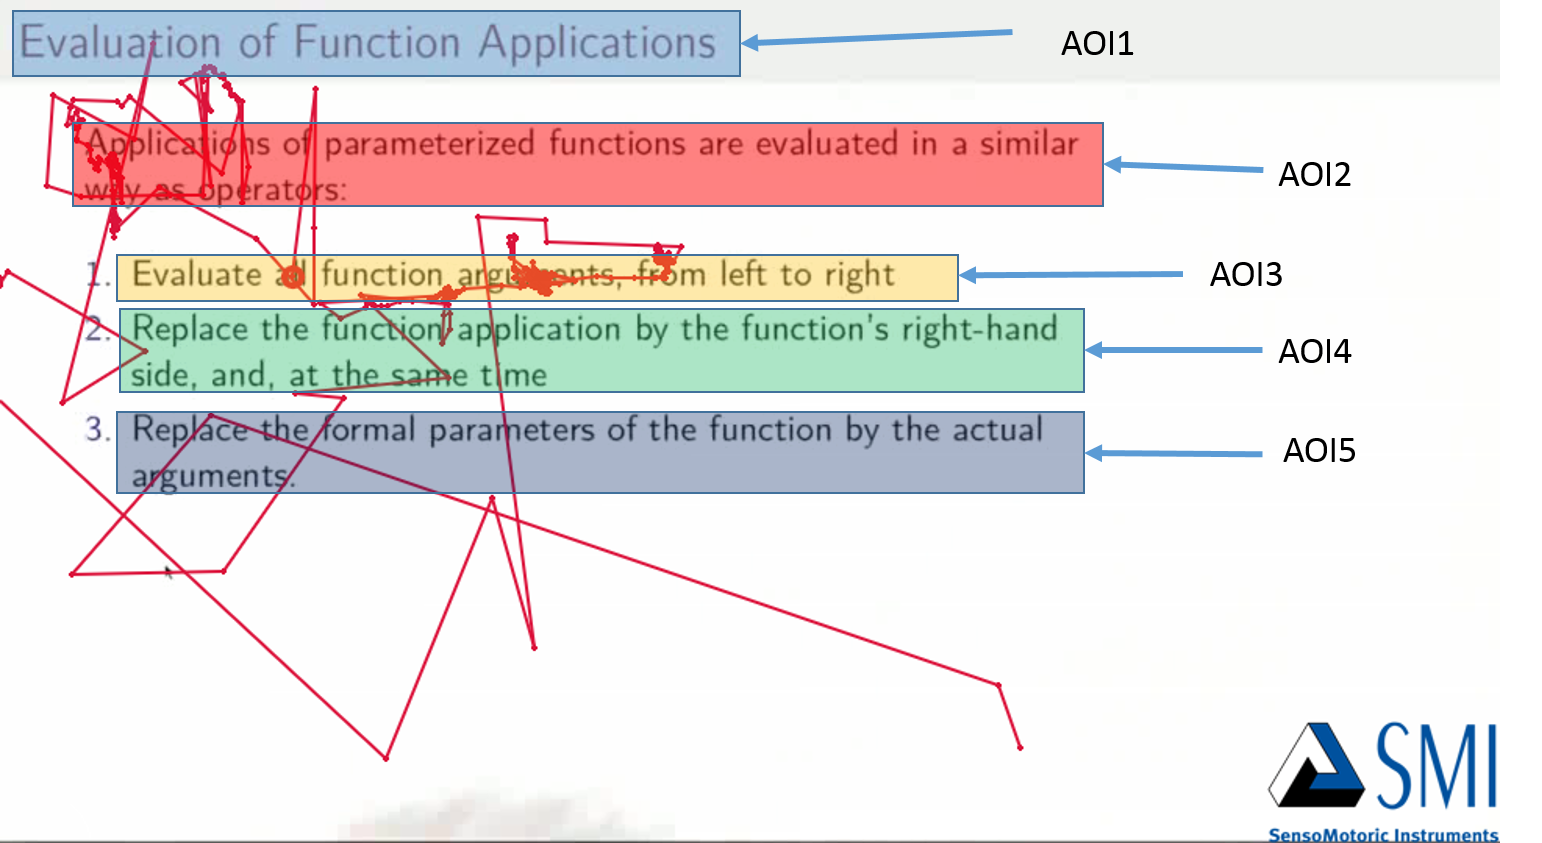
\includegraphics[width=\linewidth]{scanpathVars}
    \caption{Example of dividing a screen in Areas of interest and the saccades (red lines). Source: \cite{sharma2014how}}
    \label{aoi}
\end{figure}


 \textbf {Heat maps}: Heat maps are classical data visualisation tools. In terms of visualising eye-tracking data the heat maps show the distribution of the gaze. The distribution of the gaze then can be analysed for different user classes (for usability studies), experimental conditions or task based performance (Figure \ref{heatMap} ). The mathematical details about how to create the heat maps can be found in \cite{duchowski2007eye}. 

\begin{figure}
    \centering
    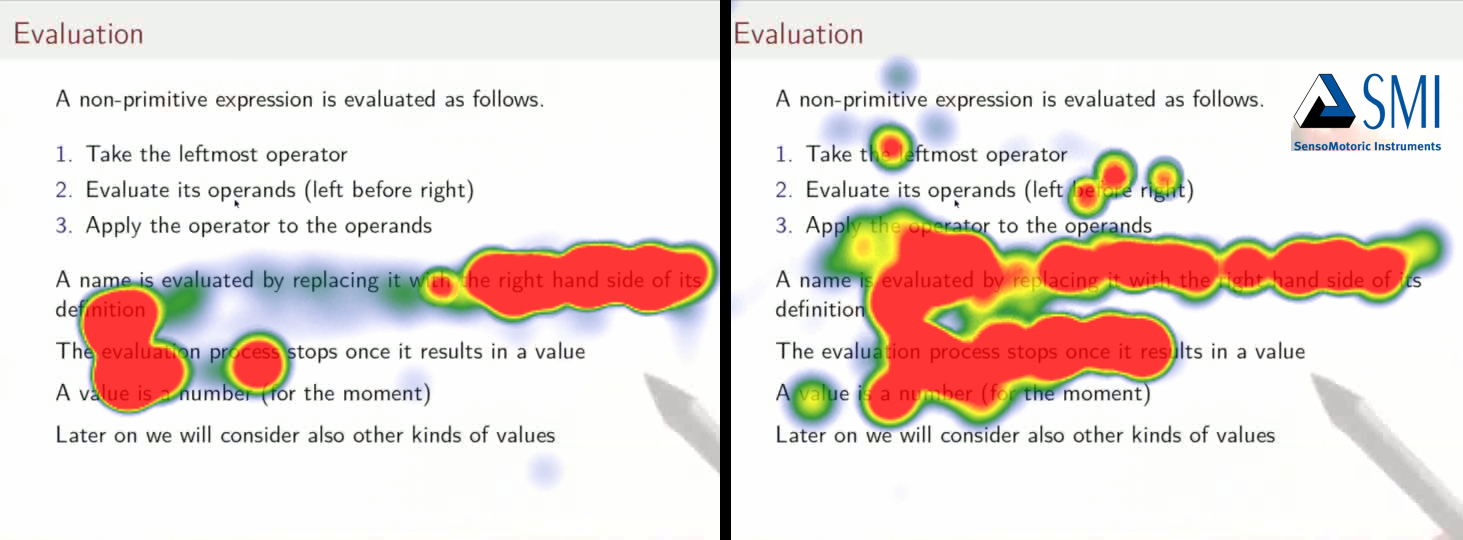
\includegraphics[width=\linewidth]{heat-map}
    \caption{Left : Example heat map for a MOOC student who performed poor in the posttest. Right: Example heat map for a MOOC student who performed well in the posttest. Source: \cite{sharma2014how}}
    \label{heatMap}
\end{figure}





\subsection{Analysing social behaviour}

Dual eye-tracking is more complicated to analyse than the solo eye-tracking, for the sole reason of the social dimension being involved in the users' behaviour. Following are the two main points to keep in mind while analysing the social behaviour of a collaborating pair of users: 



 \textbf {Joint attention}: Maintaining common grounds among the collaborators is key to success during collaboration. This is achieved via references to the objects visible by both the participants in a pair. There are two events that create a moment of joint attention: 1) eye-voice span \cite{griffin2000eyes}: the referencing partner looks at the referred site before referring to it; and 2) voice-eye span \cite{allopenna1998tracking}: after the reference the non-referencing partner looks at the referred site. These moments of joint attention help them to create the common ground in the first place and further, they help in maintaining the common ground. The time lag between the speaker's gaze and listener's gaze at the referred object is called \emph{gaze cross recurrence} \cite{richardson2007art}. The gaze cross recurrence has been shown to be correlated with the collaboration quality and joint task performance \cite{nussli2011dual}.


 \textbf {Interaction episodes:} Apart from moments of joint attention, collaboration contains sequence of actions and communicative moves. To build a model of the interaction quality, it is essential to put temporal markers in the flow of interaction. \cite{sharma2012gaze} defined the segments of interaction by detecting \emph{stable} (looking at a small set of objects) and \emph{together} (looking at the same set of objects) moments. Simply put, for automatic assessment of quality of interaction, we need to automatically segment the interaction based on gaze data. It is important to keep in mind that different level of gaze aggregation can help in finding evidences for different granularities of task decomposition.



\subsubsection{Use cases for mobile eye-tracking} 

Mobile eye-tracking is  useful when the target and/or the observer is moving, or the experimental setup requires one or both of them to move. For example, in child-robot interaction situations, we can use mobile eye-trackers to see how much the child look at the robot and what are the actions robot does which attract most of the child's attention. Also in the case of robots designed for the elderly and demented people we could assess the effects of robots' actions on the gaze of the users.

Having the target and/or the  observer moving may result in having partial target in the field of view of the observer. Hence, there is a methodological problem to solve, which is "how to track the target when it is partially out of sight?" To accomplish this we need to put fiducial markers in the scene or extract some salient features of the target which make it easy to automatically locate the gaze pointer on the target and/or the scene

%%%%%%%%%%%%%%%%%%%%%%%%%%%%%%%%%%%%%%%%%%%%%%%%%%%%%%%%%%%%%%%%%%%%%%%%%%%%%%%%%%%%
%%%%%%%%%%%%%%%%%%%%%%%%%%%%%%%%%%%%%%%%%%%%%%%%%%%%%%%%%%%%%%%%%%%%%%%%%%%%%%%%%%%%

\section{Method Application Example}
\label{application}

In this section, we present a mobile eye-tracking study with an educational robot Thymio II \cite{riedo2012two}. The study exemplifies one of the use cases of the mobile eye-tracking. One part of the target (the robot) was moving, whereas the rest of the maze (or playground, as we refer to it in the rest of this paper) was stationary. The participants were allowed to move but most of them remained seated for the duration of the experiment.  We decided to use the mobile eye trackers to be able to have our participants freely move on the experiment site. 

\subsection{Setup and Conditions}

Thymio II is a small robot designed for education for 6 to 16 year old
children~\cite{magnenat2012programming, riedo2012two}. Users can interact with
it via buttons and distance sensors. The robot can display its states via 
LEDs and its motion. We programmed it to show the value of the front IR-sensor
on its top. The display consists of 8 LEDs (Figure~\ref{thymio}).

In the experiment, there were 3 sensor data visualisation conditions.  For the
{\sf TRUE} visualisation condition, the number of illuminated LEDs, on the top of the
robot, is proportional to the intensity measured by the IR-sensor. When the
intensity of the reflected IR crosses a predefined threshold, the robot does a
90° turn to its right. For the two other conditions, the behaviour is the same,
simply the display changes. In the {\sf RANDOM} condition, the display shows as if the
robot was detecting the obstacle at random moments, while in the {\sf NONE}
visualization condition nothing is shown on top of the robot. The robot has a
fitting for a pencil that we used for the drawing of its trajectory.

\begin{figure}
    \centering
    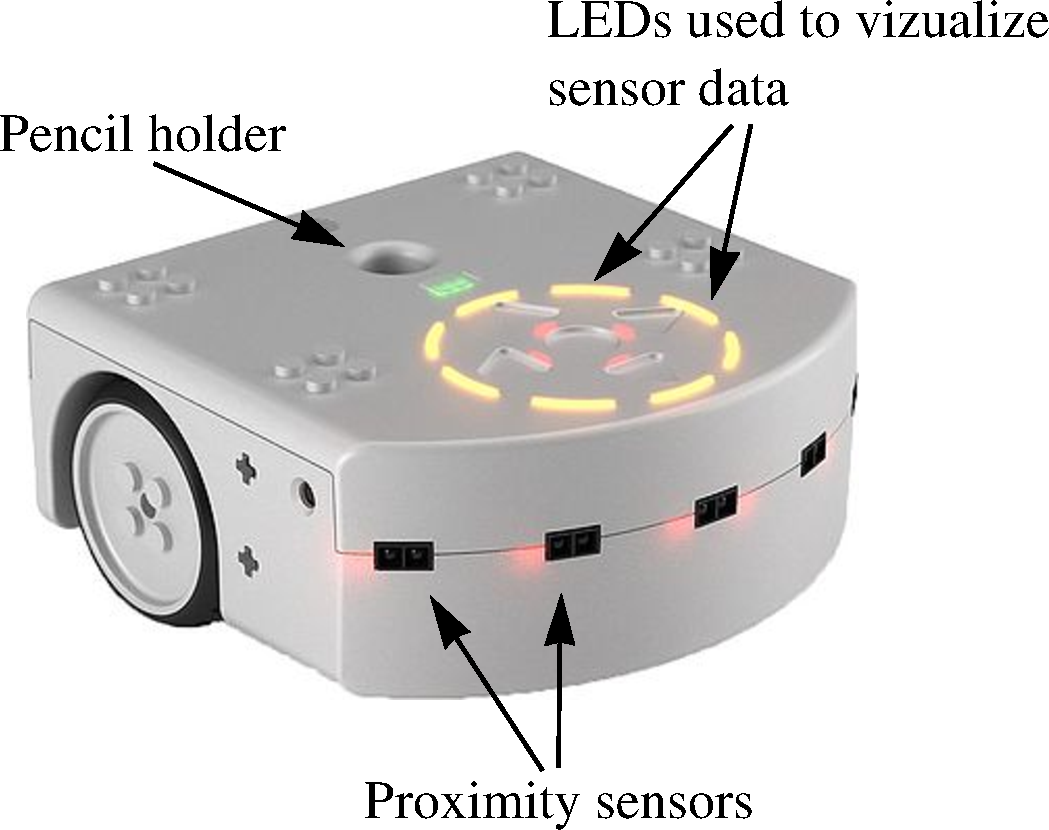
\includegraphics[width=0.9\linewidth]{thymio}
    \caption{\small \textbf{Thymio II}: the proximity sensors were used to
    detect the obstacle based on the reflectance of the material. The sensor
    data was shown as a proportion of the circle lit using the LEDs on top of the
    robot.}

    \label{thymio}
\end{figure}

The playground (Figure~\ref{playground}) is designed in order to allow the
participants to get a reference of the previous behaviour of the robot, as well
as to allow us to localise the position of the robot, the position of the
obstacles and the position of the gaze on the video recorded from the
eye-tracker.  On the right hand side, the observation phase takes
place and there will be the reference for the black and white obstacles. On the
left hand side, the interaction takes place.

\begin{figure}
    \centering
    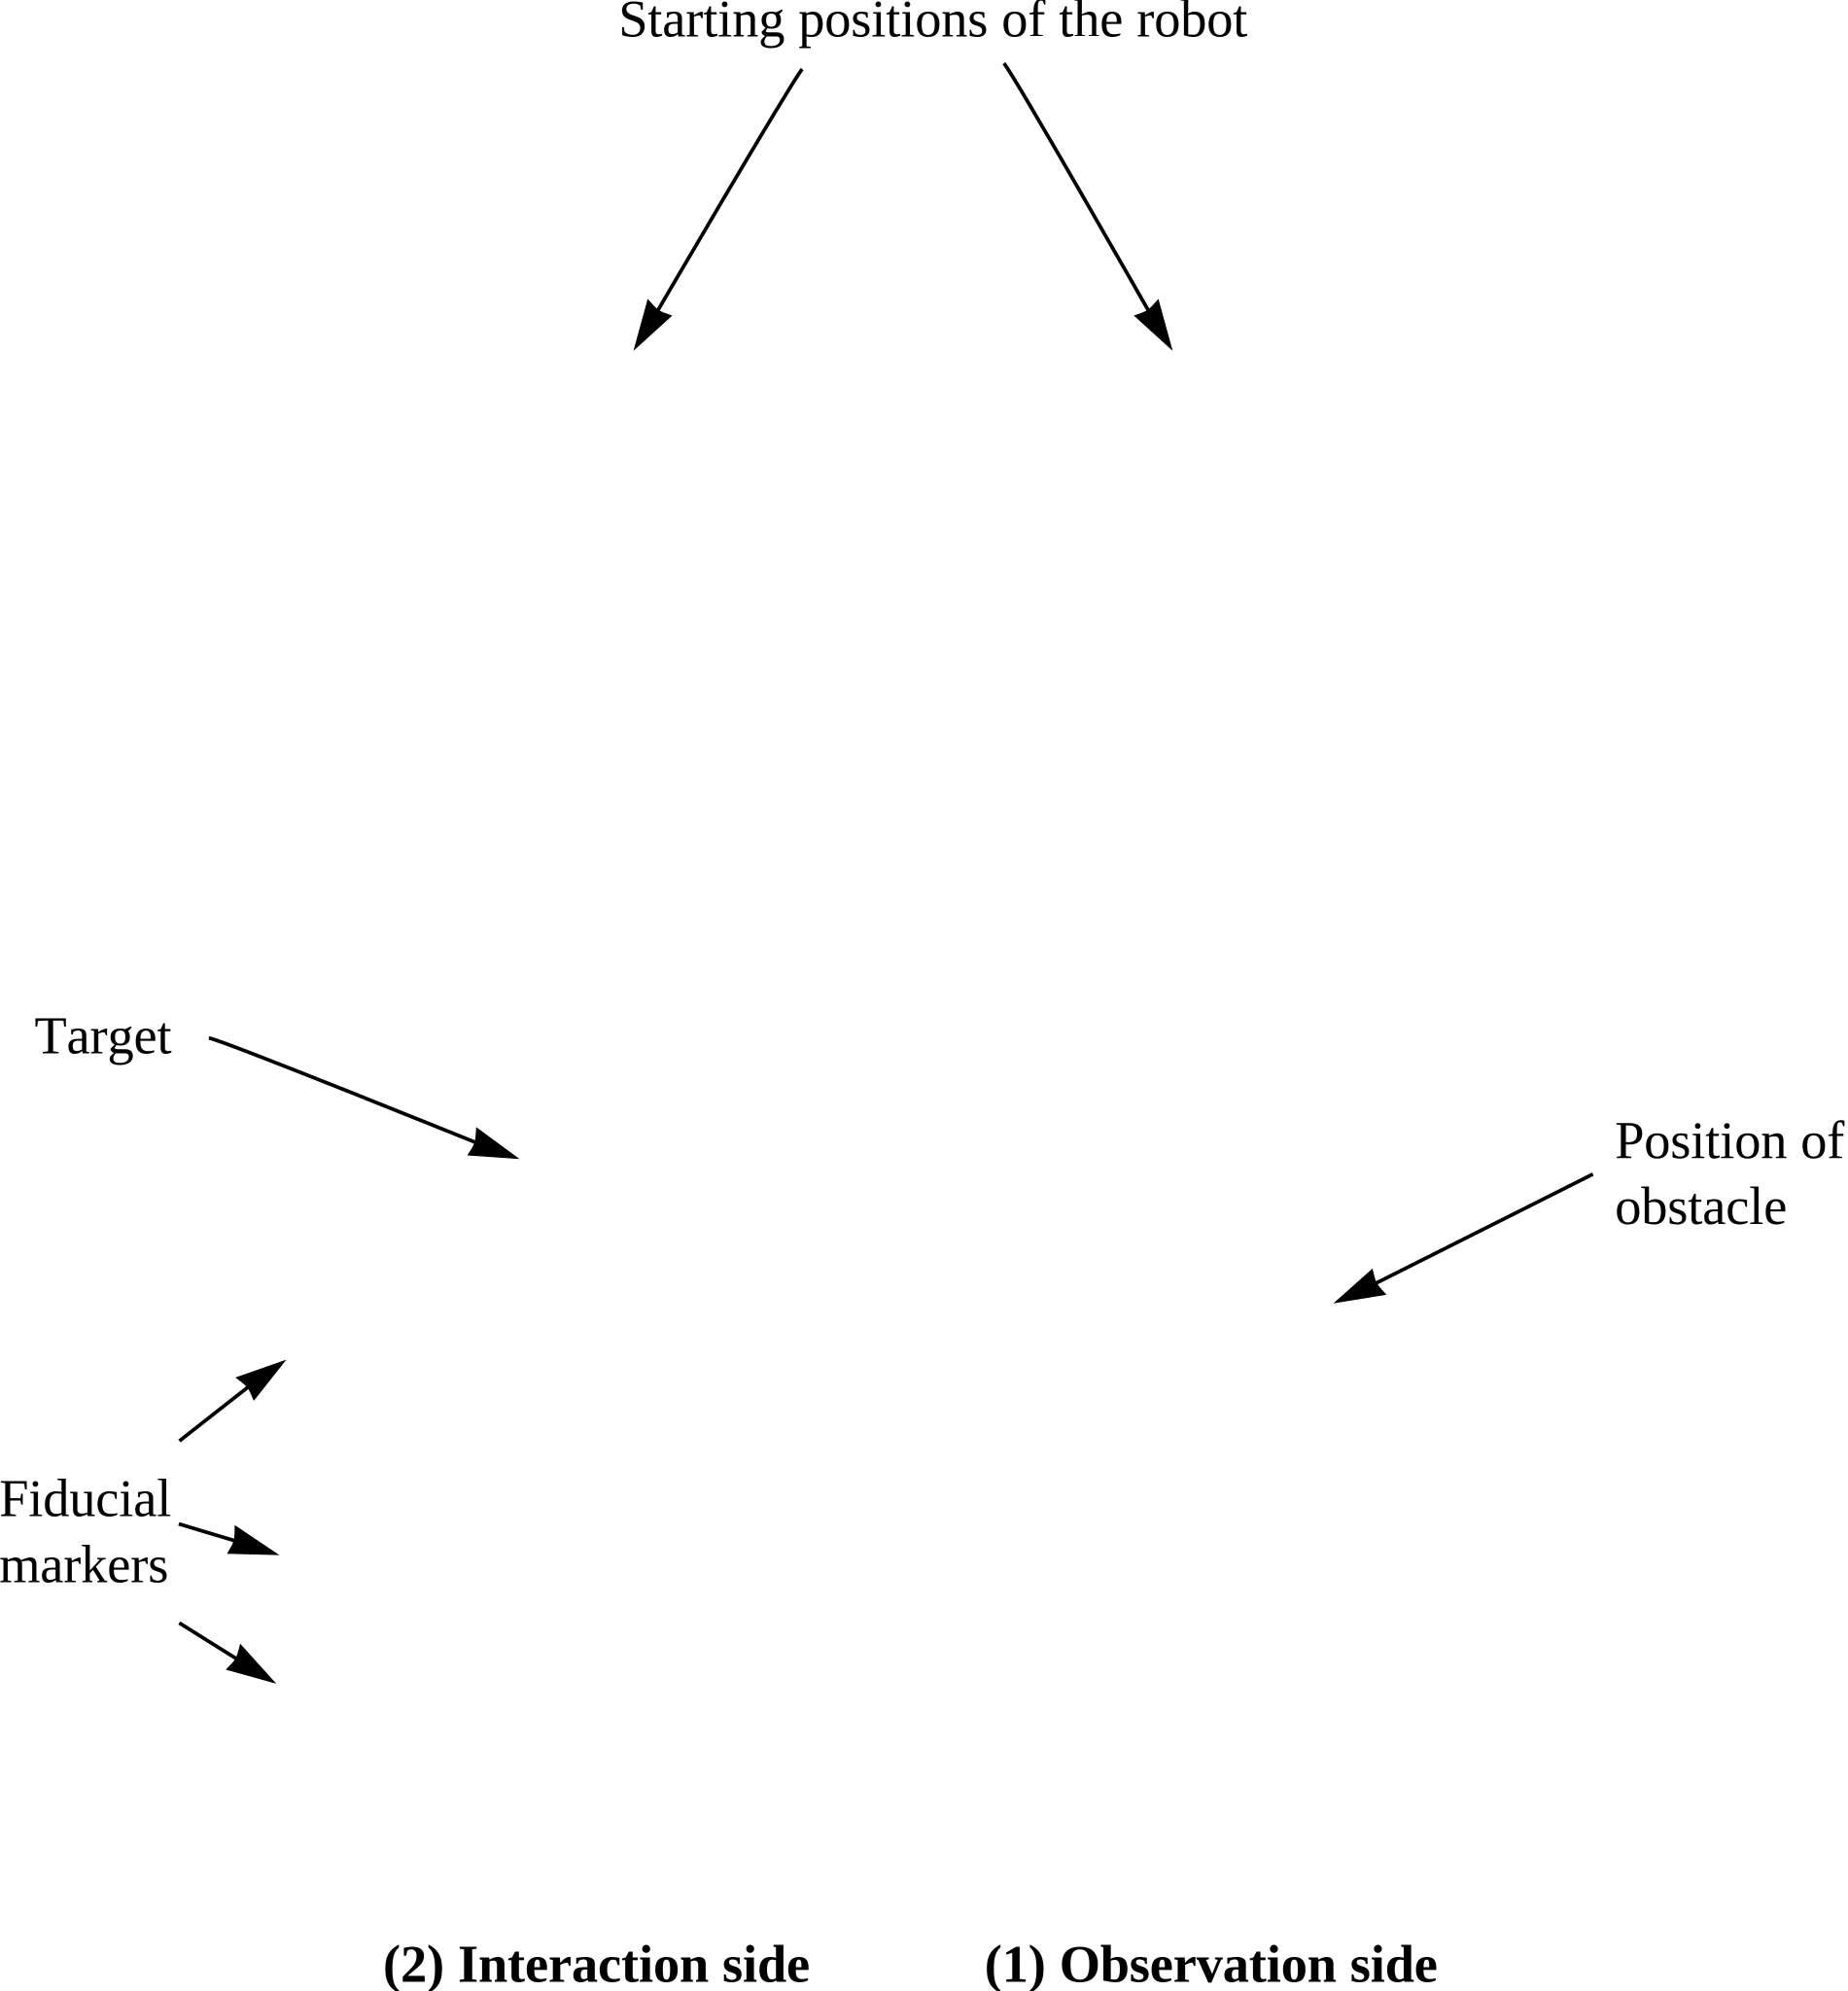
\includegraphics[width=0.9\linewidth]{maze}
    \caption{\small Basic playground for the experiment. The fiducial markers
    are used for automatic localisation of the gaze pointers on the observation
    video.}

    \label{playground}
\end{figure}

One important fact to be considered is that the localisation of the
robot, the obstacle or the gaze pointer on the observation field for the
participant is not a trivial task. The fact that the participants are
free to move, poses a challenge to the eye-tracking analysis. The
movement of the participant causes change in the observation field of
the participant almost every frame of the eye-tracking video. To cope up
with the changing observation field we decided to put an array of
fiducial markers on the playground. Using the fiducial markers enabled
us to recreate the whole playground for every frame in the video
recorded from the eye-tracker's camera (Figure~\ref{playground}).

\subsection{Procedure and Participants}

We recruited 52 participants for the experiment. All of them were
students from ANONYMOUS, ANONYMOUS. The participants were placed in front of the playground (Figure~\ref{expe}) and were
equipped with the SMI eye-tracking glasses. The eye-tracker records the gaze
data at 30Hz with an accuracy of 0.5 degrees at 40 centimetres distance; and the
scene camera of the eye-tracking glasses records the video in HD.  The actual
experiment consisted in two phases: observation phase and interaction phase.

\paragraph{Observation phase} The participant observes the Thymio II robot
approaching obstacles. The robot turns as soon as it detects the
obstacle. The participant watches the robot's behaviour for a black and a
white obstacle for 5 trials each. For the white, the robot turns
earlier; for the black obstacle the robot turns later. In the final
trial the robot is equipped with a pen to draw its trajectory for both
obstacles with different colours. After drawing, the participant is asked
the question: ``How does the robot work?''

\paragraph{Interaction phase} In the second phase, the participant is asked
to guide the robot to a goal, using a grey obstacle. The participant can put the
obstacle wherever he likes on the left hand side (Figure~\ref{playground}) of
the playground before the robot starts. We designed the grey obstacle to reflect
more infrared light (IR) than the black or the white obstacles therefore the
robot turns even earlier. This leads to a surprising effect. The participant has
only the robot's trajectories as a source of information. Each participant is
given 5 trials to put the obstacle in order to guide the robot to the goal. The
participant then has to answer the same question as in the observation phase,
response to which is considered as a final answer.

\begin{figure}
    \centering
    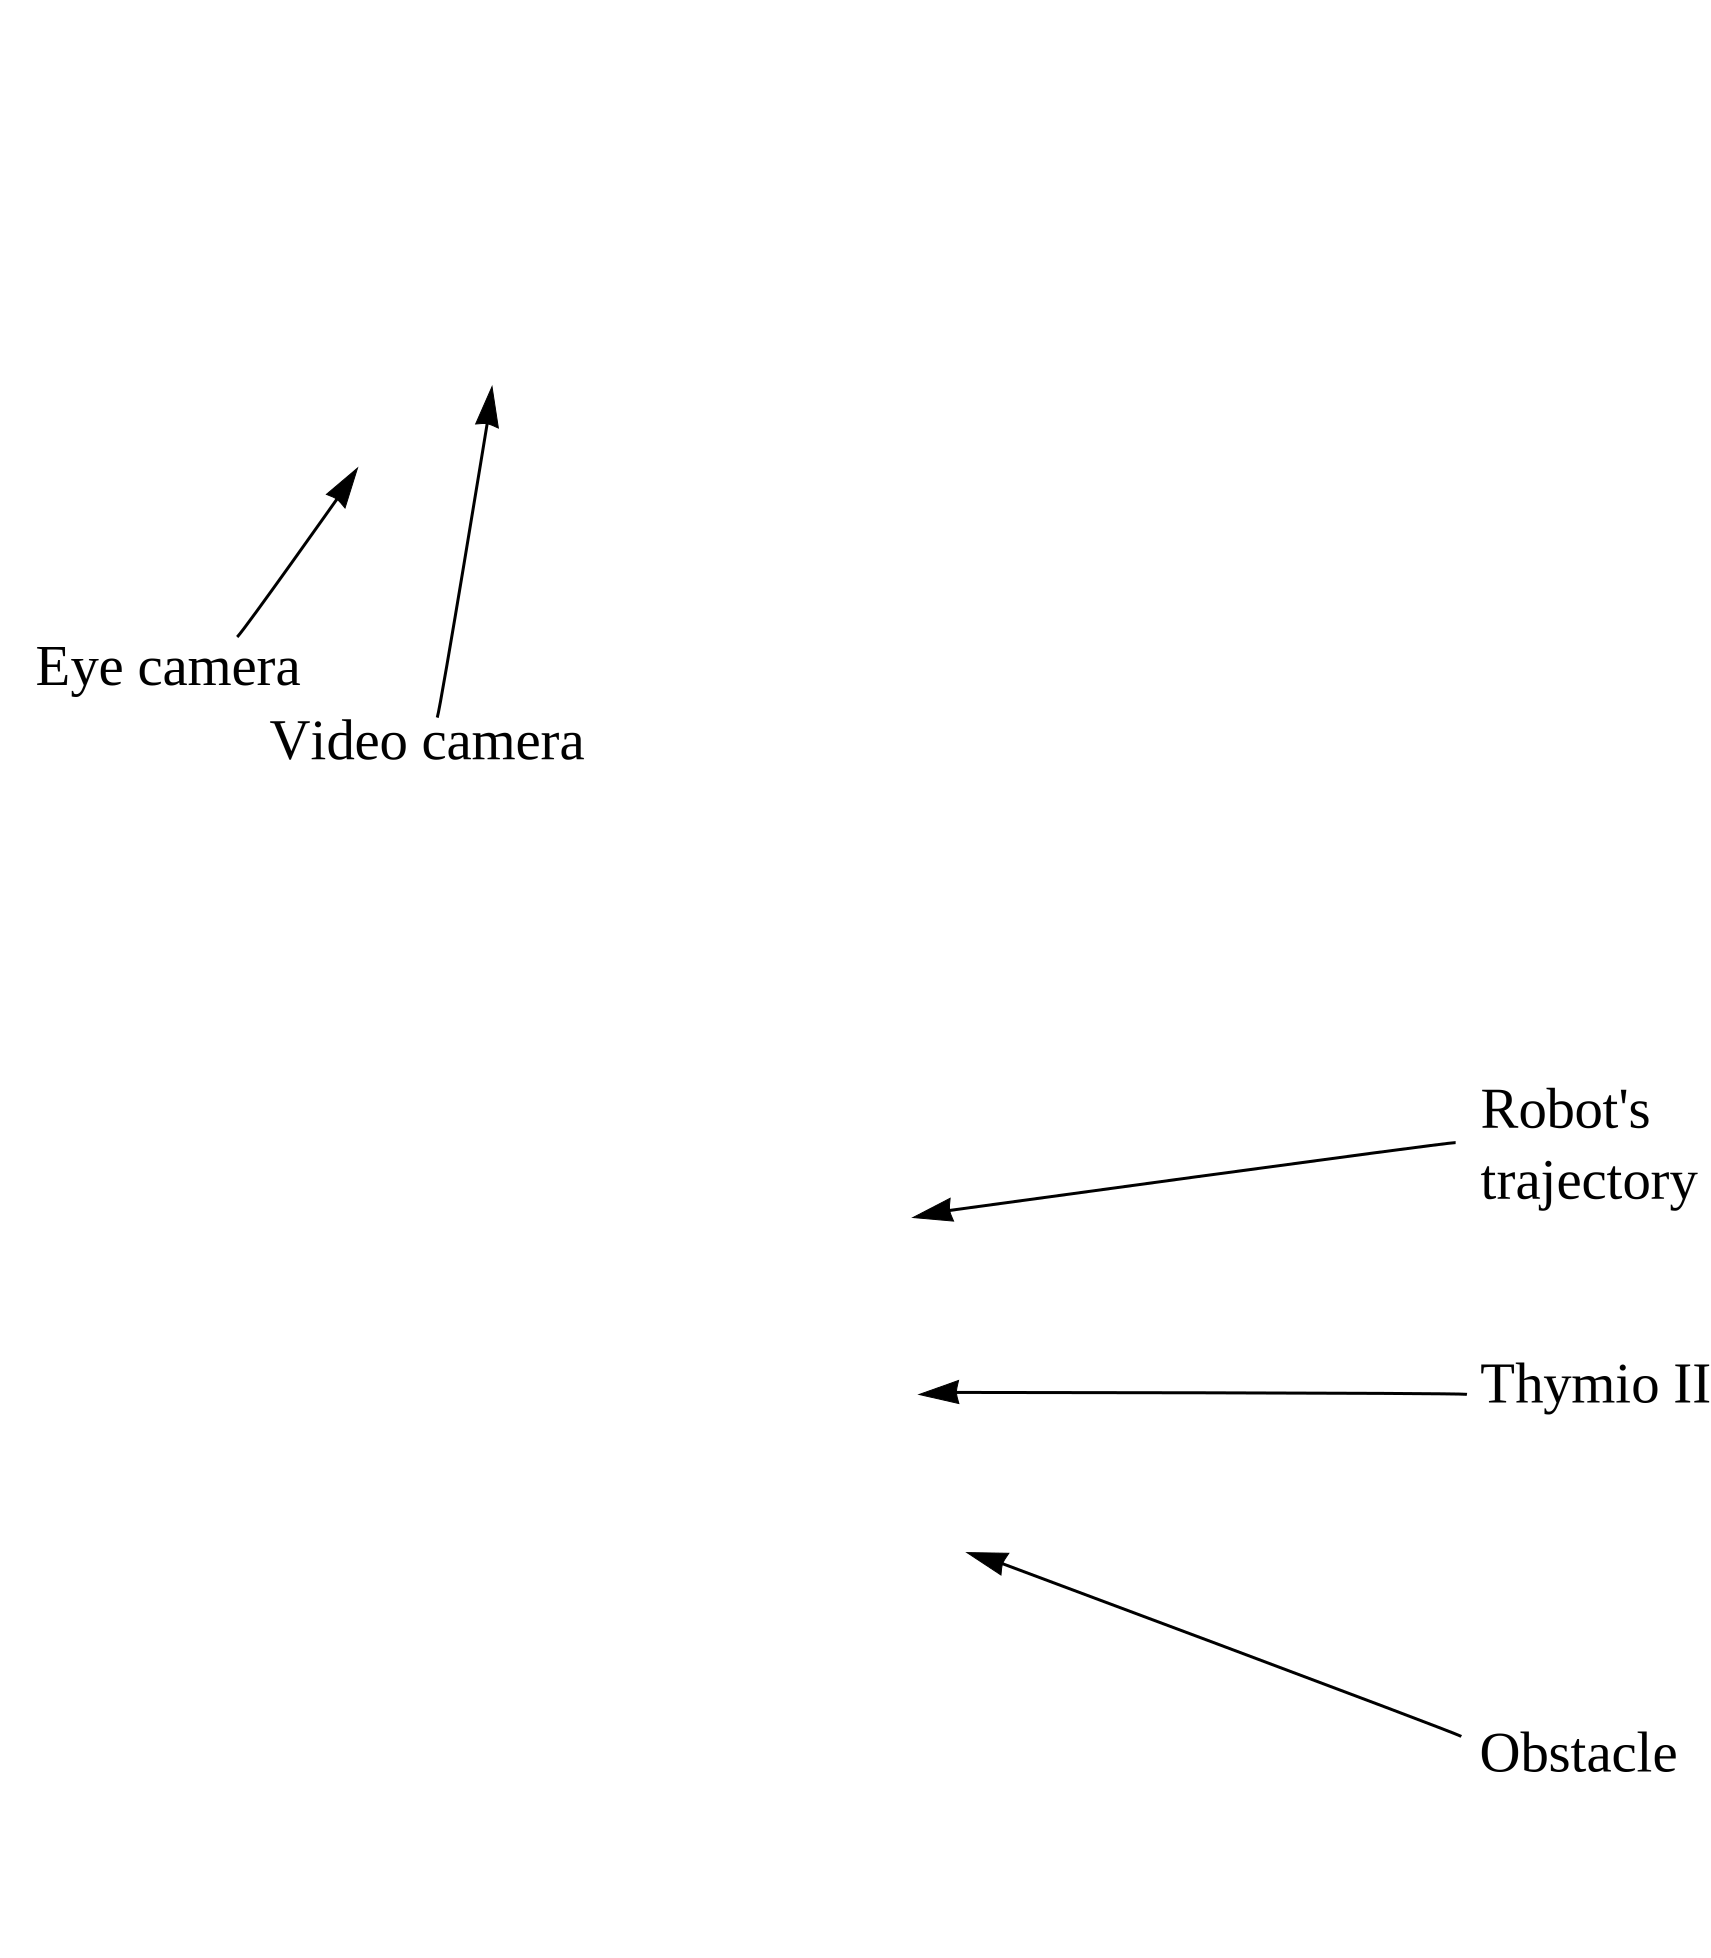
\includegraphics[width=0.9\linewidth]{setup}
    \caption{\small Experimental setup for observation phase. The observation
    video is recorded from the video camera in the front of the eye tracker (in
    the lop-left corner).}

    \label{expe}
\end{figure}


\subsection{Eye-tracking measures}

Average fixation duration on the robot: We measured the amount of time a
participant looks at the robot and averaged this duration for the number
of fixations on the robot for the particular participant.

Average fixation on the reference side: The main area (right hand side
of figure \ref{playground}) in the observation phase is treated as the reference side
in the interaction phase. The rationale behind keeping the lines drawn
by the robot in the observation phase is for the participants to be able
to refer to the prior behaviour of the robot in the interaction phase. We
measured the amount of time a participant looks at the reference side
and averaged this duration for the number of fixations on the reference
side for the particular participant.

\subsection{Performance measures}


We measured the distances from the target for all 5 trials. As soon as the principle of the robot was deemed to be understood by the participants, almost all the participants behaved the same way. On the first try almost every participant failed with the robot turning instantly. So the most significant distance measure was the
improvement between the first and second trial. It is referred to as improvement in the next section.



%%%%%%%%%%%%%%%%%%%%%%%%%%%%%%%%%%%%%%%%%%%%%%%%%%%%%%%%%%%%%%%%%%%%%%%%%%%%%%%%%%%%
%%%%%%%%%%%%%%%%%%%%%%%%%%%%%%%%%%%%%%%%%%%%%%%%%%%%%%%%%%%%%%%%%%%%%%%%%%%%%%%%%%%%

\section{Results and Interpretation}
\label{interpretation}

In this section, we give some of the results form the study which illustrate how fixations can be used to analyse the behaviours during the human-robot interaction and the cognitive constructs can be supported with the results.

\subsection{Results}

First, we show how fixation durations can be used to compare the experimental conditions and the task based performance levels.

\paragraph{Average fixation duration on the robot during observation phase
vs.~condition}

The average fixation duration on the robot during observation phase
(Figure~\ref{res1}) is significantly more in {\sf TRUE} and {\sf RANDOM} condition than in
the {\sf NONE} condition ($F[2,49]=3.68$, p = .03). This shows that the
sensor data visualisation has an effect on the users' attention.

\begin{figure}[h!]
    \centering
    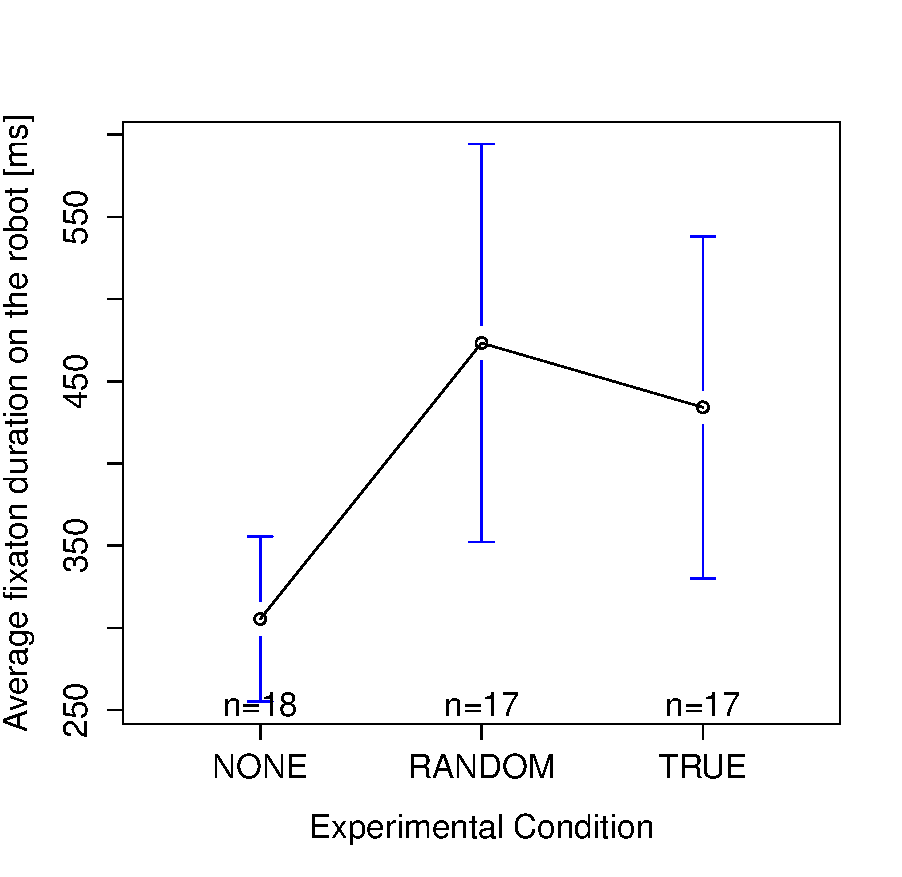
\includegraphics[width=0.8\linewidth]{meanPlotFixRobo}
    \caption{Average fixation duration on the robot ~during the observation phase
    vs.~Condition}
    \label{res1}
\end{figure}

\paragraph{First improvement vs.~condition}

The first improvement is significantly more in {\sf NONE} and {\sf RANDOM}
conditions (Figure~\ref{res2}) than in the {\sf TRUE} condition ($F[2,49]=3.75$, p =
0.03).

\begin{figure}[h!]
    \centering
    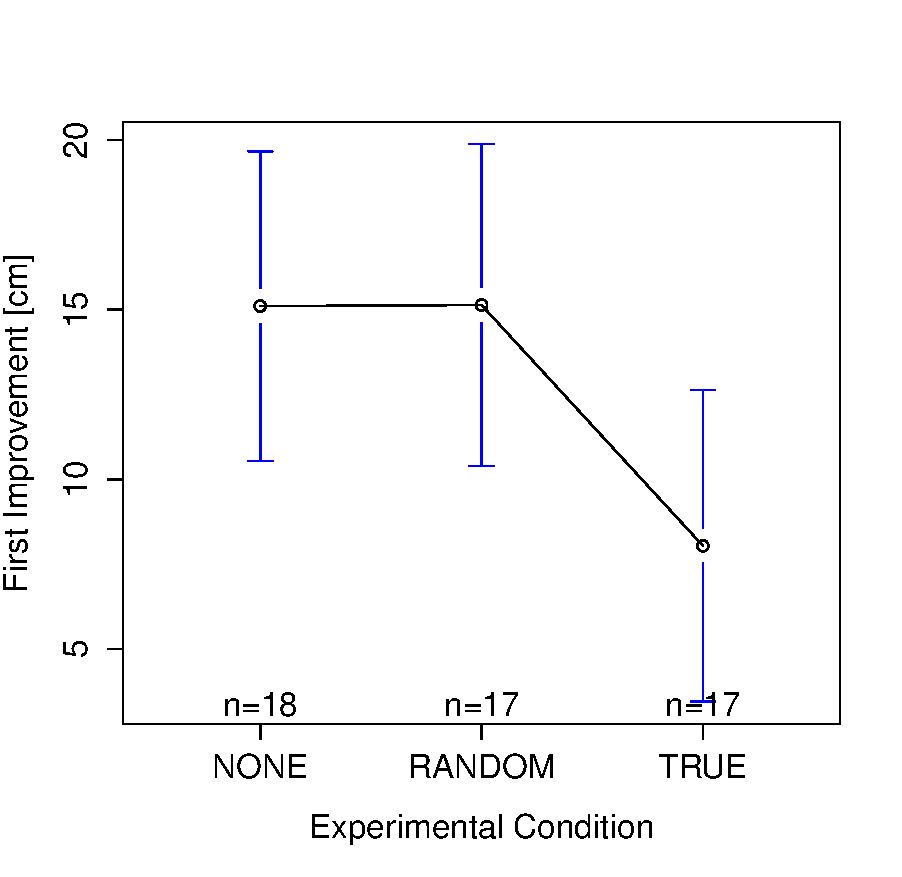
\includegraphics[width=0.8\linewidth]{meanPlotFirstImprove}
    \caption{First improvement vs.~experimental condition}
    \label{res2}
\end{figure}

\paragraph{Average fixation duration on the reference side during interaction
phase vs.~condition}

The average fixation time on the reference side of the playground
(Figure~\ref{res3}) during the interaction phase is significantly more in {\sf NONE}
and {\sf RANDOM} condition than it is in the {\sf TRUE} condition ($F[2,49]=4.19$,
p = .02).

\begin{figure}[h!]
    \centering
    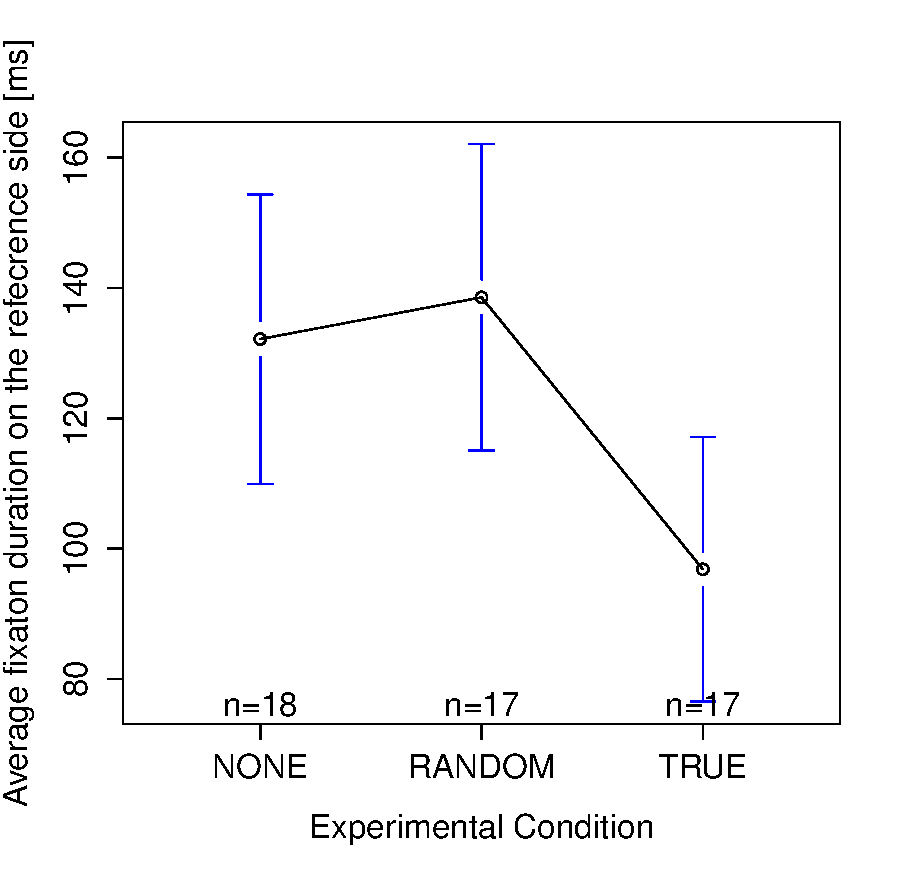
\includegraphics[width=0.8\linewidth]{meanPlotFixReference}
    \caption{Average fixation duration on the reference side during the
    interaction phase vs.~Condition}
    \label{res3}
\end{figure}

\paragraph{First improvement vs number of fixations on reference side}

Now we show how we can use the fixation counts on different areas of interest to analyse the different task based performance levels. There is a significant negative correlation between the number of
fixations on the reference side (Figure~\ref{res4}) during the interaction phase
and the first Improvement ($t(50)=-2.13$, Pearson's correlation = -0.29, p=.03).

\begin{figure}[h!]
    \centering
    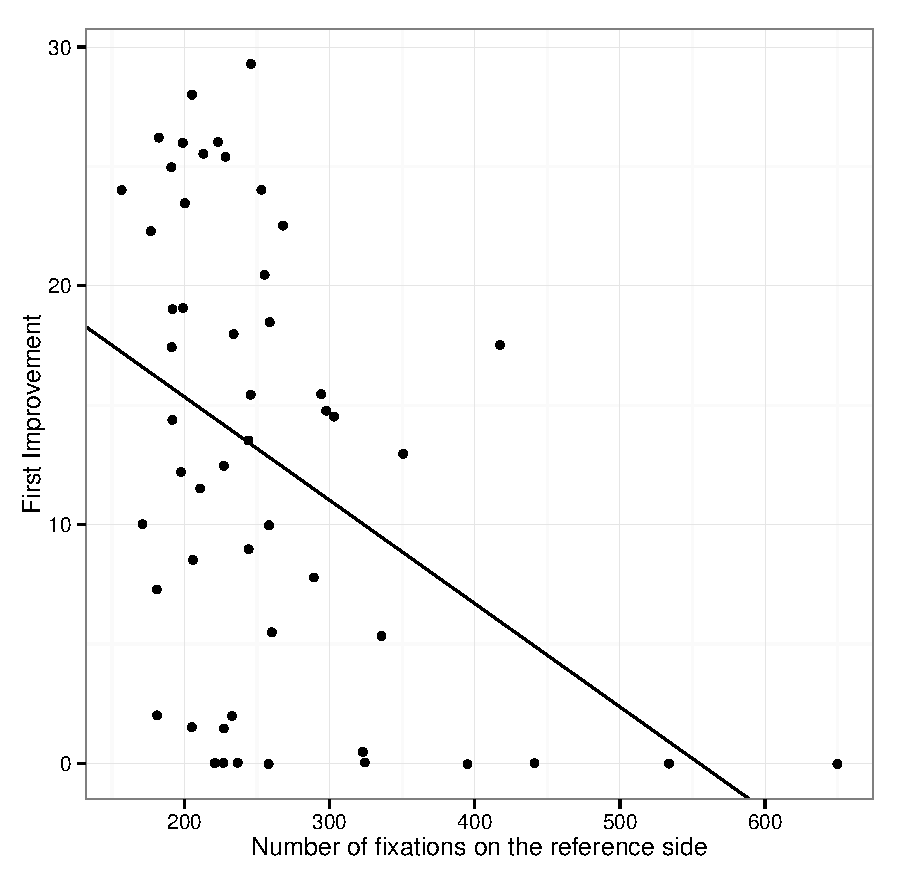
\includegraphics[width=0.8\linewidth]{corPlotFirstImprove}
    \caption{First improvement in centimeters ($y$-axis) vs.~number of fixations
    on reference side ($x$-axis) during the interaction phase.}
    \label{res4}
\end{figure}

%%%%%%%%%%%%%%%%%%%%%%%%%%%%%%%%%%%%%%%%%%%%%%%%%%%%%%%%%%%%%%%%%%%%%%%%%%%%%%%%%%%%
%%%%%%%%%%%%%%%%%%%%%%%%%%%%%%%%%%%%%%%%%%%%%%%%%%%%%%%%%%%%%%%%%%%%%%%%%%%%%%%%%%%%

\subsection{Interpretation}

The fact that participants have
higher average fixation duration on the robot during the observation phase in
the {\sf NONE} condition than the other two conditions (Figure 4) is not
surprising as displaying visual information on the robot induces a saliency
effect on the attention and the gaze is attracted towards the salient feature in
the field of view. 

The fact that the participants in the {\sf RANDOM} or {\sf NONE} visualisation
condition improved more than those with {\sf TRUE} condition is surprising
(Figure 5). There are two plausible explanations. The first is that participants
who see the robot in the {\sf TRUE} condition have a stronger belief that the
robot always behaves the same. They see the LEDs of the robot turning on and
therefore the robot still works. The ones with {\sf NONE} visualisation do not
have an indication whether the robot works the same way as in the observation
phase, and start experimenting earlier. The second explanation is that the
participants in {\sf TRUE} condition just put the obstacles out of detection
range, because they could see different display information and concluded
therefore it may behave differently.

The fact that participants have lower average fixation duration on the
reference side in the interaction phase in the {\sf TRUE} condition than the
other two conditions actually supports the explanation that participants
with {\sf TRUE} condition had a higher initial belief in their cognitive model
of how does the robot work (Figure 6). They did not need to look onto
the reference given in observation phase. This also verifies our working
hypothesis that a carefully designed mapping between the robot's
behaviour and its visual actuators can help in maximising the learning
effect during the interaction. It is important to highlight the fact that the previous two interpretations combine the behaviour of the participants, the experimental condition and the gaze measures. Thus eye-tracking provide a strong tool to form and verify cognitive hypotheses to interpret the social behaviour in human-robot interaction.

We can also have a similar interpretation from the relation between the fixation counts and the first improvement. The fact that there is a negative correlation  between the number of
fixations on the reference side (Figure~\ref{res4}) during the interaction phase
and the first Improvement also reflects that those participants who had higher belief in their initial mental models did not look at the reference side in the interaction phase and failed in the first trial. 
%%%%%%%%%%%%%%%%%%%%%%%%%%%%%%%%%%%%%%%%%%%%%%%%%%%%%%%%%%%%%%%%%%%%%%%%%%%%%%%%%%%%
%%%%%%%%%%%%%%%%%%%%%%%%%%%%%%%%%%%%%%%%%%%%%%%%%%%%%%%%%%%%%%%%%%%%%%%%%%%%%%%%%%%%

\section{Conclusion}
\label{conclusion}

The robotic task that we have just presented was initially motivated by those
two questions:

\begin{enumerate}
    \item Can we \emph{characterise} the participants' behaviours that
        lead to good performance during the interaction? In particular, do
        we observe any higher cognitive skills like anticipation patterns for
        the good performers?

    \item How do visual cues affect the performance of the participants?

\end{enumerate}

We indeed were interested in accessing and understanding the cognitive
mechanisms at stake during the interaction: where do participants look when they
want to understand a robot behaviour? Does \emph{anticipation} for instance
reflect understanding? How the robot's design impact the interaction? These kind
of questions are common in HRI, and we believe that mobile eye-tracking, as a
relatively non-invasive yet accurate (both spatially and temporally) biometric
measurement, is a valuable tool to investigate them in ecologically
valid environments.

We identify three main strengths of eye-tracking. First, eye-tracking introduces
less experimental bias: mobile eye-tracker are non-invasive and lightweight.
Combined with mobile recording units, they do not put any constraints on
participant movements, contrary to traditional techniques like video recording.
Also, contrary to questionnaires or interview-based protocols where the
experimenter's active role may influence the participants' answers, eye-trackers
are easy to ``forget about'' for the participants.

Second, eye-tracking provides a direct, un-mediated access to the subject's
attentional focus~\cite{sharma2014withmeness} (both spatially -- where does the
subject look at -- and temporally -- where does the subject's attention remain).
Importantly, this information can be implicitly interpreted as a fine-grained measure of
\emph{engagement}.  Also, the good temporal resolution of eye-trackers allows
for the accurate study of the \emph{dynamics} of attention, including possible
\emph{attentional patterns} of the subject during the interaction.

Third, it has been shown in literature that eye-tracking can provide an
effective measure of higher socio-cognitive behaviours: it can be used as a
predictor for successful joint task achievement~\cite{sharma2013understanding},
or as a measure of \emph{interaction quality}~\cite{jermann2012effects} through
measurement of joint attention.

One need however to be aware of its limitations: eye-tracking does not give a direct
access to underlying mental representations, and a gaze pattern does not
automatically tell us what the subject think of (EEG or fMRI may be slightly
closer to that target, but they come with their own range of limitations).

Besides, mobile eye-tracking come with an additional cost. As we mentioned
earlier, the automatic localisation of the gaze pointer on the visual stimulus
is not a trivial task. In our study, we relied on a number of fiducial markers
to the playground, but they were reported as distractive by the participants.
More complex computer vision tools (like object tracking) can alleviate the need
for such markers, but it certainly requires significant pre-processing prior to
data analysis.

Still, we believe that eye-tracking, as a method for the assessment and
understanding of the complex cognitive mechanisms that underlie human-robot
interaction, is a promising tool, currently under-used in robotics.



%%%%%%%%%%%%%%%%%%%%%%%%%%%%%%%%%%%%%%%%%%%%%%%%%%%%%%%%%%%%%%%%%%%%%%%%%%%%%%%%%%%%
%%%%%%%%%%%%%%%%%%%%%%%%%%%%%%%%%%%%%%%%%%%%%%%%%%%%%%%%%%%%%%%%%%%%%%%%%%%%%%%%%%%%
% Removed for double-blind review
%\section*{Acknowledgments}
%
%This research was supported by...

%%%%%%%%%%%%%%%%%%%%%%%%%%%%%%%%%%%%%%%%%%%%%%%%%%%%%%%%%%%%%%%%%%%%%%%%%%%%%%%%%%%%
%%%%%%%%%%%%%%%%%%%%%%%%%%%%%%%%%%%%%%%%%%%%%%%%%%%%%%%%%%%%%%%%%%%%%%%%%%%%%%%%%%%%
\bibliographystyle{abbrv}
\bibliography{eyetracking}

\balancecolumns

\end{document}

